\documentclass[11pt]{article}

% Pacchetti utili
\usepackage[utf8]{inputenc}  
\usepackage{amsmath}         
\usepackage{amssymb}         
\usepackage{graphicx}        
\usepackage{geometry}        
\usepackage{fancyhdr}        
\usepackage{hyperref}       
\usepackage{float} 
\usepackage{xcolor}
\usepackage{tabularx}

% Impostazioni per i margini
\geometry{a4paper, margin=0.8in}
% Spaziatura tra righe
%\linespread{0.9}

% Grandezza righe tabelle
\renewcommand{\arraystretch}{1.2} % Aumenta l'altezza delle righe

% Intestazioni
\pagestyle{fancy}
\fancyhf{}
\fancyhead[L]{Linguaggi Formali e Compilatori}
\fancyhead[R]{Soluzione Esercizi Tipo - Parte II}
\fancyfoot[C]{\thepage}   


\begin{document}
\section{Esercizio 1}

\subsection{Creazione dell'automa caratteristico}
Creiamo l'automa caratteristico $\cal A$ per il parsing bottom-up SLR(1). Iniziamo aggiungendo 
una nuova produzione con un nuovo non terminale che produce lo start symbol: 
$$ S'\rightarrow \cdot S $$ 
Procediamo con il calcolo della chiusura LR(0), che consiste nell'includere 
tutte le produzioni in cui il non terminale preceduto dal marker funge da 
driver, e ripetiamo questo processo in modo ricorsivo, ottenendo così il 
risultato finale:
$$ S \rightarrow \cdot AaB\;|\;\cdot b $$
$$ A \rightarrow \cdot BcBaA \; | \; \cdot $$
$$ B \rightarrow \cdot $$
Questo sarà lo stato iniziale 0 dell'automa. Analizzando le transizioni da 
questo stato, otteniamo i seguenti kernel degli stati di arrivo:

\begin{itemize}
  \item Transizione con $S$: il kernel è $\{ S' \rightarrow S \cdot \}$, corrispondente allo stato 1. 
  La chiusura di questo stato è vuota poiché il marker ($\cdot$) si trova alla fine della produzione, 
  rendendo questo stato reducing (stato finale). Inoltre, questo stato è anche lo stato di accettazione.
  
  \item Transizione con $A$: il kernel è $\{ S \rightarrow A \cdot aB \}$, corrispondente allo stato 2. 
  Anche in questo caso, la chiusura è vuota perché il marker non precede alcun non terminale.
  
  \item Transizione con $b$: il kernel è $\{ S \rightarrow b \cdot \}$, corrispondente allo stato 3. 
  La chiusura è vuota e, essendo uno stato reducing, è anche uno stato finale.
  
  \item Transizione con $B$: il kernel è $\{ A \rightarrow B \cdot cBaA \}$, corrispondente allo stato 4.
  La chiusura di questo stato è vuota.
\end{itemize}

\noindent Notiamo che lo stato 0 ha due item di riduzione $A \rightarrow \cdot$ e $B \rightarrow \cdot$, 
quindi è anche uno stato finale. Proseguendo analogamente alla creazione degli altri stati seguendo le 
transizioni da quelli appena calcolati otteniamo l'automa seguente:

\begin{figure}[H]
  \centering
  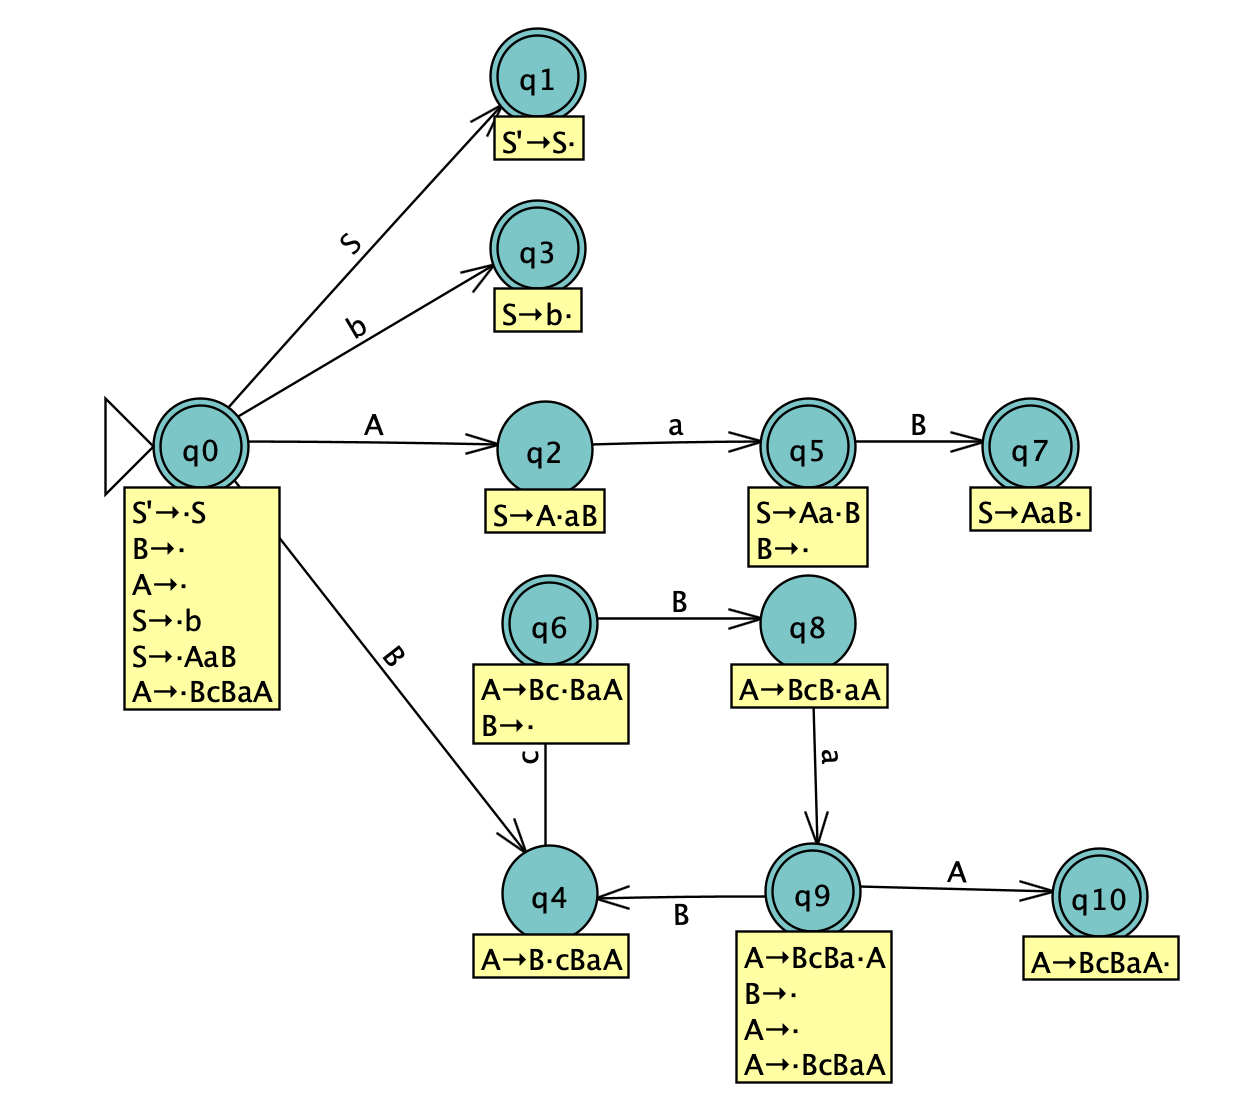
\includegraphics[width=0.7\textwidth]{img/01AutomaSRL.png}
  \label{fig:automa}
\end{figure}

\subsection{Creazione della tabella di parsing SLR(1)}
Calcoliamo i set di \textit{first} e \textit{follow}:

\begin{table}[H]
\centering
\begin{tabular}{|c|c|c|}
\hline
\textbf{Non Terminale} & \textbf{First} & \textbf{Follow} \\
\hline
$S$ & $\{a, b, c\}$ & $\{\$\}$ \\
\hline
$A$ & $\{c, \epsilon\}$ & $\{a\}$ \\
\hline
$B$ & $\{\epsilon\}$ & $\{c, a, \$\}$ \\
\hline
\end{tabular}
\label{tab:first-follow}
\end{table}

\noindent Costruiamo ora la tabella di parsing. Le transizioni dei terminali sono \textit{shift}, quelle 
dei non terminali sono \textit{GOTO}, mentre le riduzioni avvengono nei \textit{Follow} dei reducing items.

\noindent Reducing items:
\begin{itemize}
  \item $R_1$: $S \rightarrow AaB \cdot$
  \item $R_2$: $S \rightarrow b \cdot$
  \item $R_3$: $A \rightarrow BcBaA \cdot$
  \item $R_4$: $A \rightarrow \cdot$
  \item $R_5$: $B \rightarrow \cdot$
\end{itemize}

\begin{table}[H]
  \centering
  \begin{tabularx}{\textwidth}{|>{\centering\arraybackslash}X|>{\centering\arraybackslash}X|>{\centering\arraybackslash}X|>{\centering\arraybackslash}X|>{\centering\arraybackslash}X|>{\centering\arraybackslash}X|>{\centering\arraybackslash}X|>{\centering\arraybackslash}X|}
  \hline
  \textbf{Stato} & \textbf{a} & \textbf{b} & \textbf{c} & \textbf{\$} & \textbf{A} & \textbf{B} & \textbf{S} \\
  \hline
  0 & \colorbox{yellow}{R4 / R5} & S3 & R5 & R5 & 2 & 4 & 1 \\
  \hline
  1 &  &  &  & acc &  &  & \\
  \hline
  2 & S5 &  &  &  &  &  & \\
  \hline
  3 &  &  &  & R4 &  &  &  \\
  \hline
  4 &  &  & S6 &  &  &  & \\
  \hline
  5 & R5 &  & R5 & R5 &  & 7 & \\
  \hline
  6 & R5 &  & R5 & R5 &  & 8 & \\
  \hline
  7 &  &  &  & R1 &  &  & \\
  \hline
  8 & S9 &  &  &  &  &  & \\
  \hline
  9 & \colorbox{yellow}{R4 / R5} &  & R5 & R5 & 10 & 4 & \\
  \hline
  10 & R3 &  &  &  &  &  & \\
  \hline
  \end{tabularx}
  \label{tab:parsing}
\end{table}

\subsection{Risposte alle domande}

\begin{enumerate}
  \item Gli stati dell'automa $\cal A$ sono 11.
  \item Le mosse di shift sono 4.
  \item Le mosse di reduce sono 17.
  \item Sono presenti due conflitti evidenziati in giallo nella tabella.
  \item I conflitti sono:
  \begin{itemize}
    \item $T\big[I, a\big]$: conflitto \textit{reduce/reduce}, produzioni coinvolte: $A\rightarrow \epsilon$ e $B\rightarrow \epsilon$.
    \item $T\big[I[BcBa], a\big]$: conflitto \textit{reduce/reduce}, produzioni coinvolte: $A\rightarrow \epsilon$ e $B\rightarrow \epsilon$.
  \end{itemize}
\end{enumerate}

\newpage

\section{Esercizio 2}
\subsection{Creazione dell'automa caratteristico}
Lo svolgimento è analogo all'esercizio precedente:

\begin{figure}[H]
  \centering
  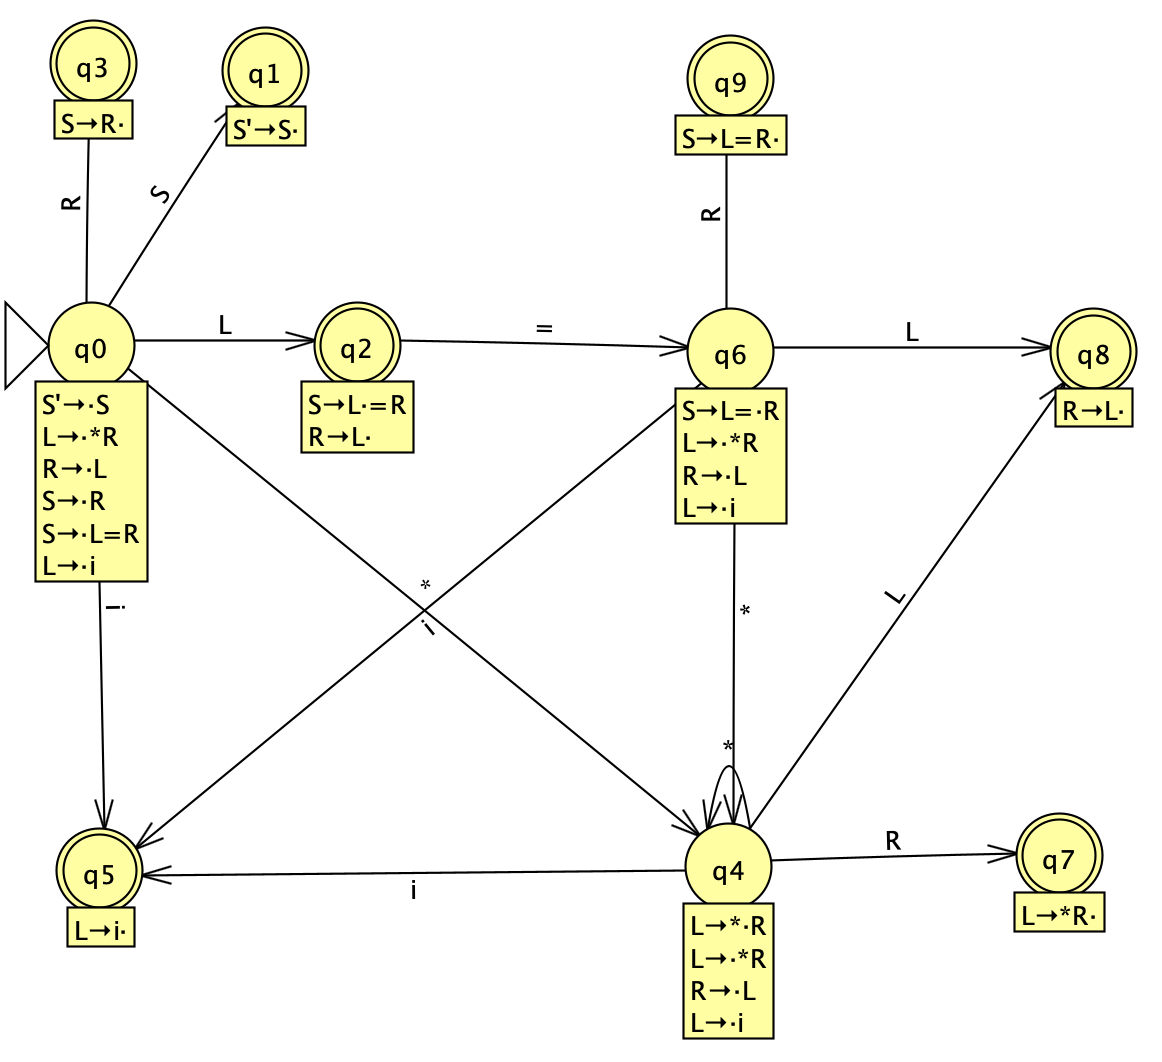
\includegraphics[width=0.7\textwidth]{img/02AutomaSRL.png}
  \label{fig:automa}
\end{figure}

\subsection{Creazione della tabella di parsing SLR(1)}
Calcoliamo i set di \textit{first} e \textit{follow}:

\begin{table}[H]
\centering
\begin{tabular}{|c|c|c|}
\hline
\textbf{Non Terminale} & \textbf{First} & \textbf{Follow} \\
\hline
$S$ & $\{*, id\}$ & $\{\$\}$ \\
\hline
$L$ & $\{*, id\}$ & $\{=, \$\}$ \\
\hline
$R$ & $\{*, id\}$ & $\{=, \$\}$ \\
\hline
\end{tabular}
\label{tab:first-follow}
\end{table}
\noindent Reducing items:
\begin{itemize}
  \item $R_1$: $S \rightarrow L=R \cdot$
  \item $R_2$: $S \rightarrow R \cdot$
  \item $R_3$: $L \rightarrow *R \cdot$
  \item $R_4$: $L \rightarrow id\cdot$
  \item $R_5$: $R \rightarrow L\cdot$
\end{itemize}
\newpage
\noindent Calcoliamo la tabella di parsing:
\begin{table}[H]
  \centering
  \begin{tabularx}{\textwidth}{|>{\centering\arraybackslash}X|>{\centering\arraybackslash}X|>{\centering\arraybackslash}X|>{\centering\arraybackslash}X|>{\centering\arraybackslash}X|>{\centering\arraybackslash}X|>{\centering\arraybackslash}X|>{\centering\arraybackslash}X|}
  \hline
  \textbf{Stato} & \textbf{*} & \textbf{=} & \textbf{id} & \textbf{\$} & \textbf{L} & \textbf{R} & \textbf{S} \\
  \hline
  0 & S4 &  & S5 &  & 2 & 3 & 1 \\
  \hline
  1 &  &  &  & acc &  &  & \\
  \hline
  2 &  & \colorbox{yellow}{S6 / R5} &  & R5 &  &  & \\
  \hline
  3 &  &  &  & R2 &  &  &  \\
  \hline
  4 & S4 &  & S5 &  & 8 & 7 & \\
  \hline
  5 & & R4 &  & R4 &  &  & \\
  \hline
  6 & S4 &  & S5 &  & 8 & 9 &  \\
  \hline
  7 &  & R3 &  & R3 &  &  & \\
  \hline
  8 &  & R5 &  & R5 &  &  & \\
  \hline
  9 &  &  &  & R1 &  &  & \\
  \hline
  \end{tabularx}
  \label{tab:parsing}
\end{table}

\subsection{Risposte alle domande}

\begin{enumerate}
  \item Gli stati dell'automa $\cal A$ sono 10.
  \item Le mosse di shift sono 7.
  \item Le mosse di reduce sono 9.
  \item E' presente un conflitto evidenziato in giallo nella tabella.
  \item $T\big[I[L], $=$\big]$: conflitto \textit{shift/reduce}, in particolare 
  sono coinvolte l'azione di \textit{shift 2} e la produzione $R\rightarrow L$
\end{enumerate}


\section{Esercizio 3}
\subsection{Soluzione}
Analiziamo i conflitti della grammatica $G_1$ data:
\begin{itemize}
  \item $\big[P[EaE], a\big]$: in questo stato, leggendo il simbolo terminale $a$, il parser può
effettuare una riduzione con la produzione $E \rightarrow EaE\cdot$ oppure eseguire 
un'operazione di \textit{shift} del terminale $a$.
La decisione determina l'associatività dell'operatore $a$. Per esempio se il parser 
eseguisse l'azione di \textit{reduce} garantirebbe l'associatività a sinistra. Questo 
conflitto può essere ignorato poiché non influisce sulla precedenza tra $a$ e $b$.
  
\item $\big[P[EbE], b\big]$: in modo analogo al caso precedente, ma relativo al terminale $b$, quindi possiamo ignorare anche questo conflitto.
    
\item $\big[P[EaE], b\big]$: in questo stato, leggendo il terminale $b$, il parser può ridurre 
con $E \rightarrow EaE\cdot$ oppure eseguire uno \textit{shift} del terminale $b$
Per assegnare una precedenza più alta all'operatore $a$ rispetto a $b$, il parser deve 
eseguire la riduzione. In questo modo, l'espressione $EaE$ viene risolta prima che 
$b$ venga processato.
  
\item $\big[P[EbE], a\big]$: in modo analogo al precedente per dare priorità 
all'operatore $a$ rispetto a $b$, il parser dovrebbe scegliere l'azione di \textit{shift}. 
In questo modo, l'operatore $a$ verrà letto e processato prima che venga effettuata la riduzione con $b$.
\end{itemize}


\subsection{Automa caratteristico}
\begin{figure}[H]
  \centering
  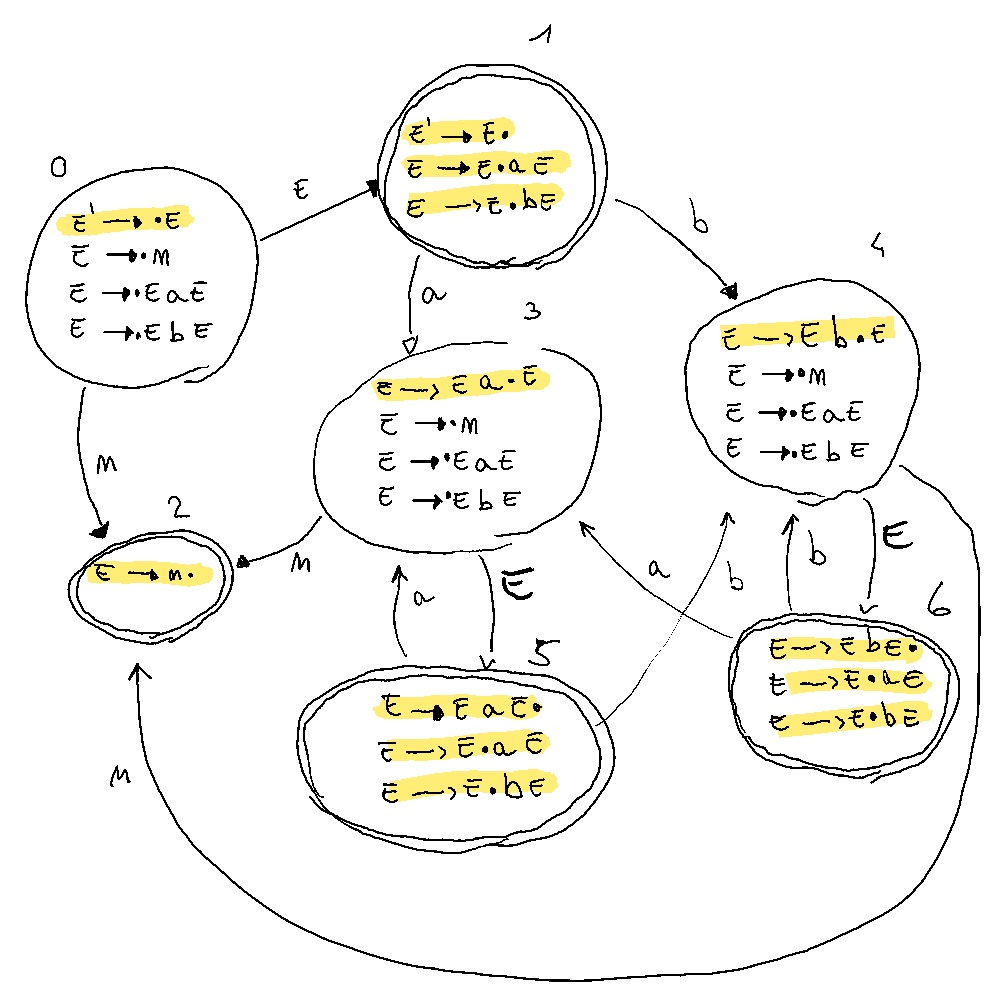
\includegraphics[width=0.7\textwidth]{img/03AutomaSRL.jpg}
  \label{fig:automa}
\end{figure}
\subsection {Tabella di parsing}

\begin{table}[H]
  \centering
  \begin{tabularx}{\textwidth}{|>{\centering\arraybackslash}X|>{\centering\arraybackslash}X|>{\centering\arraybackslash}X|>{\centering\arraybackslash}X|>{\centering\arraybackslash}X|>{\centering\arraybackslash}X|}
  \hline
  \textbf{Stato} & \textbf{a} & \textbf{b} & \textbf{n} & \textbf{\$} & \textbf{E} \\
  \hline
  0 & & & S2 & & 1 \\
  \hline
  1 & S3 & S4 & & acc & \\
  \hline
  2 & R1 & R1 &  & R1 & \\
  \hline
  3 & & & S2 & & 5\\
  \hline
  4 & & & S2 & & 6\\
  \hline
  5 & \colorbox{yellow}{S3 / R2} & \colorbox{yellow}{S4 / R2} &  & R2 &  \\
  \hline
  6 & \colorbox{yellow}{S3 / R3} & \colorbox{yellow}{S4 / R3} & & R3 &  \\
  \hline
  \end{tabularx}
  \label{tab:parsing}
\end{table}
\newpage

\section{Esercizio 4}
\subsection*{Soluzione}
Per prima cosa generiamo una nuova grammatica che tenga conto della precedenza 
dell'operatore $a$ rispetto a $b$. In particolare creiamo dei nuovi \textit{non terminali}:
\begin{itemize}
  \item $E$ rappresenterà un espressione intera
  \item $T$ rappresenterà le operazioni con priorità maggiore
  \item $F$ rappresenterà i fattori atomici o le espressioni tra parentesi 
\end{itemize}
Inoltre per garantire l'associatività a sinistra costruiremo la grammatica con ricorsione
a sinistra.
$$E \rightarrow EbT\;|\;T$$
$$T \rightarrow TaF\;|\;F$$
$$F \rightarrow (E)\;|\;id$$

\noindent Questa grammatica risolve l'ambiguità dando la precedenza all'operatore $a$ su $b$ ed è 
associativa a sinistra, ma non è LL(1), poiché presenta appunto ricorsione a sinistra.

\noindent Per eliminare la ricorsione a sinistra possiamo fattorizzare, ricordando
la formula:
$$A \rightarrow A\alpha_1 \; | \; A\alpha_2\; | \dots \; | \; \beta_1 \; |\; \beta_2\;|\; \dots$$
$$\Downarrow$$
$$A \rightarrow \beta_1 A \; |\; \beta_2 A \; | \dots$$
$$A' \rightarrow \alpha_1 A' \; | \; \alpha_2 A' \; | \; \dots \; | \; \epsilon$$

\noindent Quindi applicando la formula otteniamo:
\begin{center}
  \begin{minipage}{0.4\linewidth}
  $$E \rightarrow EbT \;|\; T$$
  $$\Downarrow$$
  $$E \rightarrow TE'$$
  $$E' \rightarrow bTE' \;| \; \epsilon$$
  \end{minipage}
  \hspace{1cm}
  \begin{minipage}{0.4\linewidth}
  $$T \rightarrow TaF \;|\; F$$
  $$\Downarrow$$
  $$F \rightarrow FT'$$
  $$T' \rightarrow aFT' \;| \; \epsilon$$
  \end{minipage}
\end{center}
Mettendo tutto insieme otteniamo:
$$E \rightarrow TE'$$
$$E'\rightarrow bTE' \;|\; \epsilon$$
$$\quad T \rightarrow FT' $$$$ T'\rightarrow aFT'\;| \epsilon$$
$$
F \rightarrow (E) \; | \; id
$$
Questa grammatica è stata vista a lezione con $b = +$ e $a = *$ e sappiamo sia LL(1).
\end{document}
